\chapter{基于自然语言模型的文件分类}

上一章在相关工作中提到,目前分层存储管理优化方式主要包括两方面:一是挖掘文件的关联性(Block Correlation),二是动态追踪应用的I/O行为并加以分析,实现I/O行为预测(热数据识别),以指导数据迁移模块进行主动的数据预取和缓存替换。以往的研究具有局限性,例如,对文件的关联性挖掘局限于目录树结构表现出的文件关系,没有对文件或目录命名隐含的语义关系予以分析;I/O行为的分析通常只针对短期内的访问规律,没有在长时间跨度上进行分析。

如图\ref{fig:model}所示,为解决上述问题,探索新的分层管理优化方式,本文使用词嵌入模型分析文件之间的语义关联,实现了文件的向量表示;在此基础上采用循环神经网络对I/O访问序列进行分析,并建立文件冷热分类模型,为分层存储中的数据迁移提供依据。
\begin{figure}[htp]
\centering
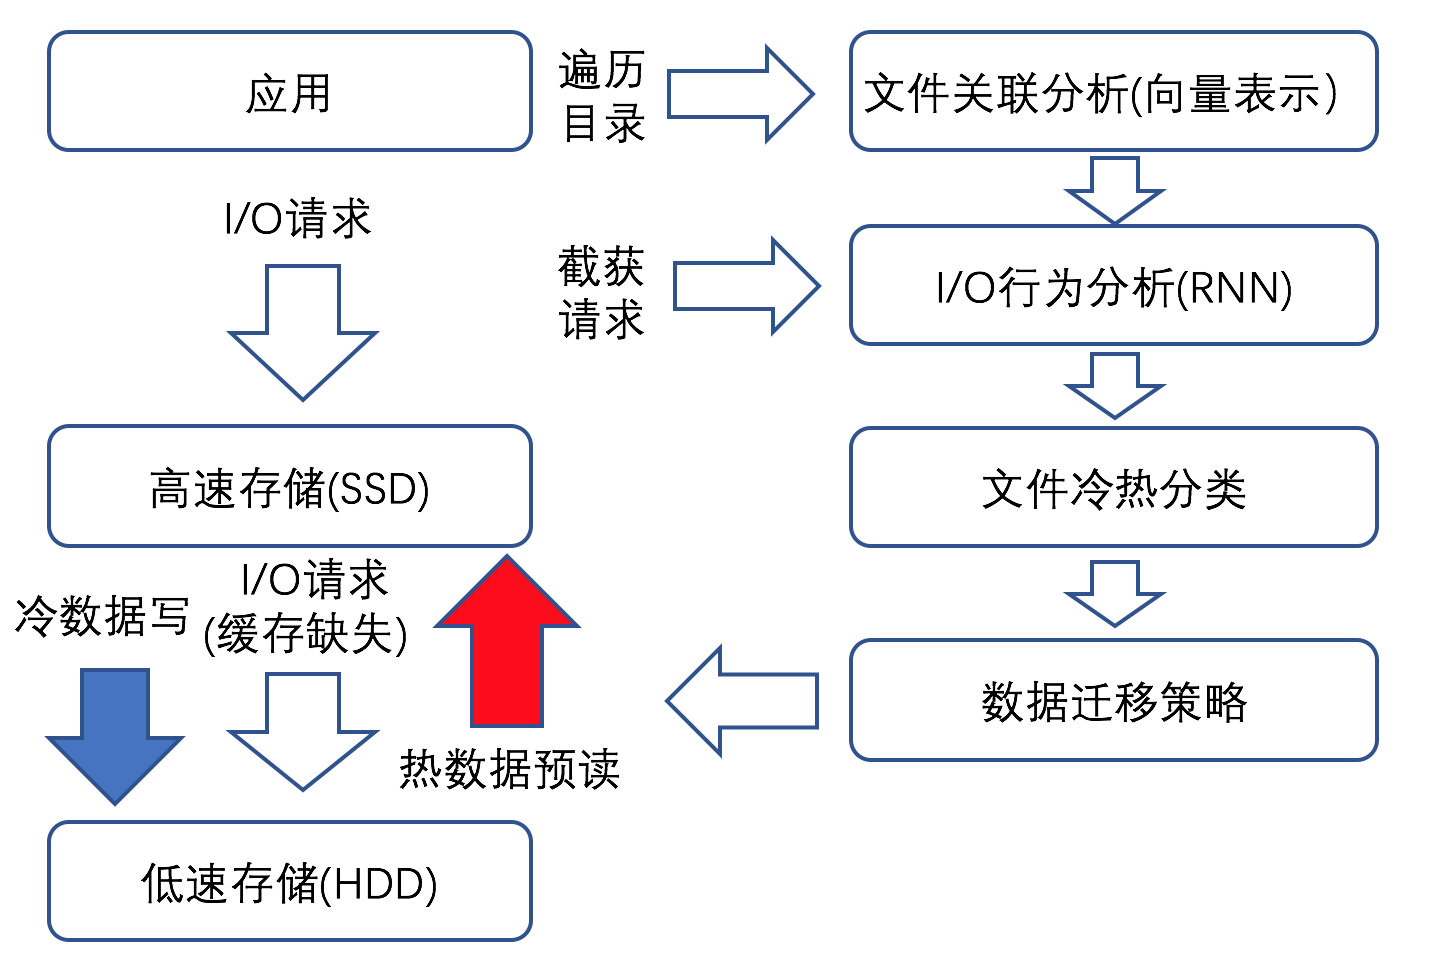
\includegraphics[width=.8\textwidth]{model}
\caption{文件分类模型设计框图}
\label{fig:model}
\end{figure}





\section{基于词嵌入模型的文件关联分析}
\subsection{文件的向量表示}
元数据(Meta Data)是指文件系统中描述数据的数据,包含数据的各种属性,例如名称、大小、类型、创建者和拥有者、以及访问权限等等,最重要的是,元数据携带用于查找定位数据的索引信息。但是,元数据通常只描述单个文件本身的属性,与其他文件的关系描述非常有限,一般只体现在目录项(directory entry)中,用于文件的逐级查找。

数据块关联(Block Correlation)在文件系统中广泛存在,且这种数据间的联系通常比较稳定,在目录结构不发生变化的情况下,一般不受工作负载的运行状态影响。反过来,工作负载访问文件的部分规律是由文件之间的固有关系决定的。如果能显示地挖掘出文件之间的联系,可以为存储系统的数据分布策略、迁移策略等提供帮助。本节将从文件之间语义关系入手,对文件关联的挖掘和表达展开研究。

以Unix文件系统为例,任意文件或目录在被创建时,均会被分配一个唯一的ID,也就是Inode序号,以此作为唯一的标识以便于后续各种文件操作。Inode序号只与文件创建先后相关,是一种one-hot的表示方式。那么能否效仿自然语言处理中词嵌入的思想,建立一种能够包含文件或目录之间关联性的表征方式?

文件系统层次结构规范(Filesystem Hierarchy Standard,FHS)\cite{fhs}是由Linux基金会在1994年发起,旨在规范Linux各发行版和其他类Unix系统下文件目录结构的业界统一标准,至今已发展演变到FHS-3.0(2015年)。在FHS定义的目录结构规范下,Linux操作系统的目录组织结构和命名受到了明确严格的约束,例如/表示根目录,/bin为系统执行文件目录,/usr/local/lib为系统函数库目录等,。如果将一个文件的完整路径(如/usr/lib/python/)视为一个句子,各级目录视为单词,下面将介绍如何使用Skip-gram模型,对给定的Unix文件系统目录下所有文件或目录进行向量表示。

1)语料库的生成

众所周知,任何机器学习模型都离不开数据,自然语言处理领域的数据集通常被称为语料库(Corpus)。任何语言学的研究或者自然语言模型的建立都必须建立在大量的语料之上,否则无论是基于规则方法还是统计方法建立的模型都将失效。

为了建立文件路径相关的“语料库”,本研究从根目录(或文件系统的挂载点)开始,通过常规的遍历算法将此目录下所有文件、目录的完整路径逐行写入到一个文本文件,作为模型的训练数据集。语料库生成后,相应地可以得到一个词汇表$V$。

2)利用Skip-gram模型训练文件与目录的词向量模型

设上文生成的语料库中单词总数为$T$,其词汇表$\mathcal{V}$=\{\textit{bin,boot,dev,...}\},词汇数量为$W$。
%其中任意一个词可用其在词汇表中的序号表示:$w \in \{1,\dots,W\}$。
那么该语料库可表示为一个由$T$个词向量组成的序列:$\mathbf{w}_1, \mathbf{w}_2, \dots, \mathbf{w}_T$。Skip-gram模型的目标就是建立一个从该词汇表中所有文件名和目录名到$d$维向量空间的映射$model:\mathcal{V} \rightarrow \mathbb{R}^d$,使以下对数极大似然函数达到最大:
\begin{equation}
    \label{eq:origin_object}
    \frac{1}{T}\sum_{t=1}^T \sum_{c \in \mathcal{C}_t} \log p(\mathbf{w}_c | \mathbf{w}_t),
\end{equation}
取负号得到损失函数:
\begin{equation}
    L(\theta)= -\frac{1}{T}\sum_{t=1}^T \sum_{c \in \mathcal{C}_t} \log p(\mathbf{w}_c | \mathbf{w}_t),
\end{equation}

其中,$\mathcal{C}_t$表示某中心词$\mathbf{w}_t$的上下文中出现过的词的集合。以路径\textit{/usr/local/lib/python}为例,若取上下文窗口大小为1,那么中心词$\mathbf{w}_t$=\textit{lib}的上下文集合$\mathcal{C}_t$=\{\textit{local,python}\},在文件系统的情境下,此处“上下文”隐含的语义是指\textit{usr},\textit{python}分别与\textit{lib}有着父子目录的关系。对于任意样本$(\mathbf{\mathbf{w}}_t,\mathbf{\mathbf{w}}_c)$,我们可用归一化函数softmax来定义单词$\mathbf{w}_c$在中心词$\mathbf{\mathbf{w}}_t$的上下文中出现的条件概率:
\begin{equation}
    \label{eq:softmax}
    p(\mathbf{w}_c | \mathbf{w}_t)=\frac{ e^{ \mathbf{w}_t^{\top} \mathbf{w}_c} }{ \sum_{j=1}^W e^{\mathbf{w}_t^{\top} \mathbf{w}_j}} 
\end{equation}

\begin{figure}[htp]
\centering
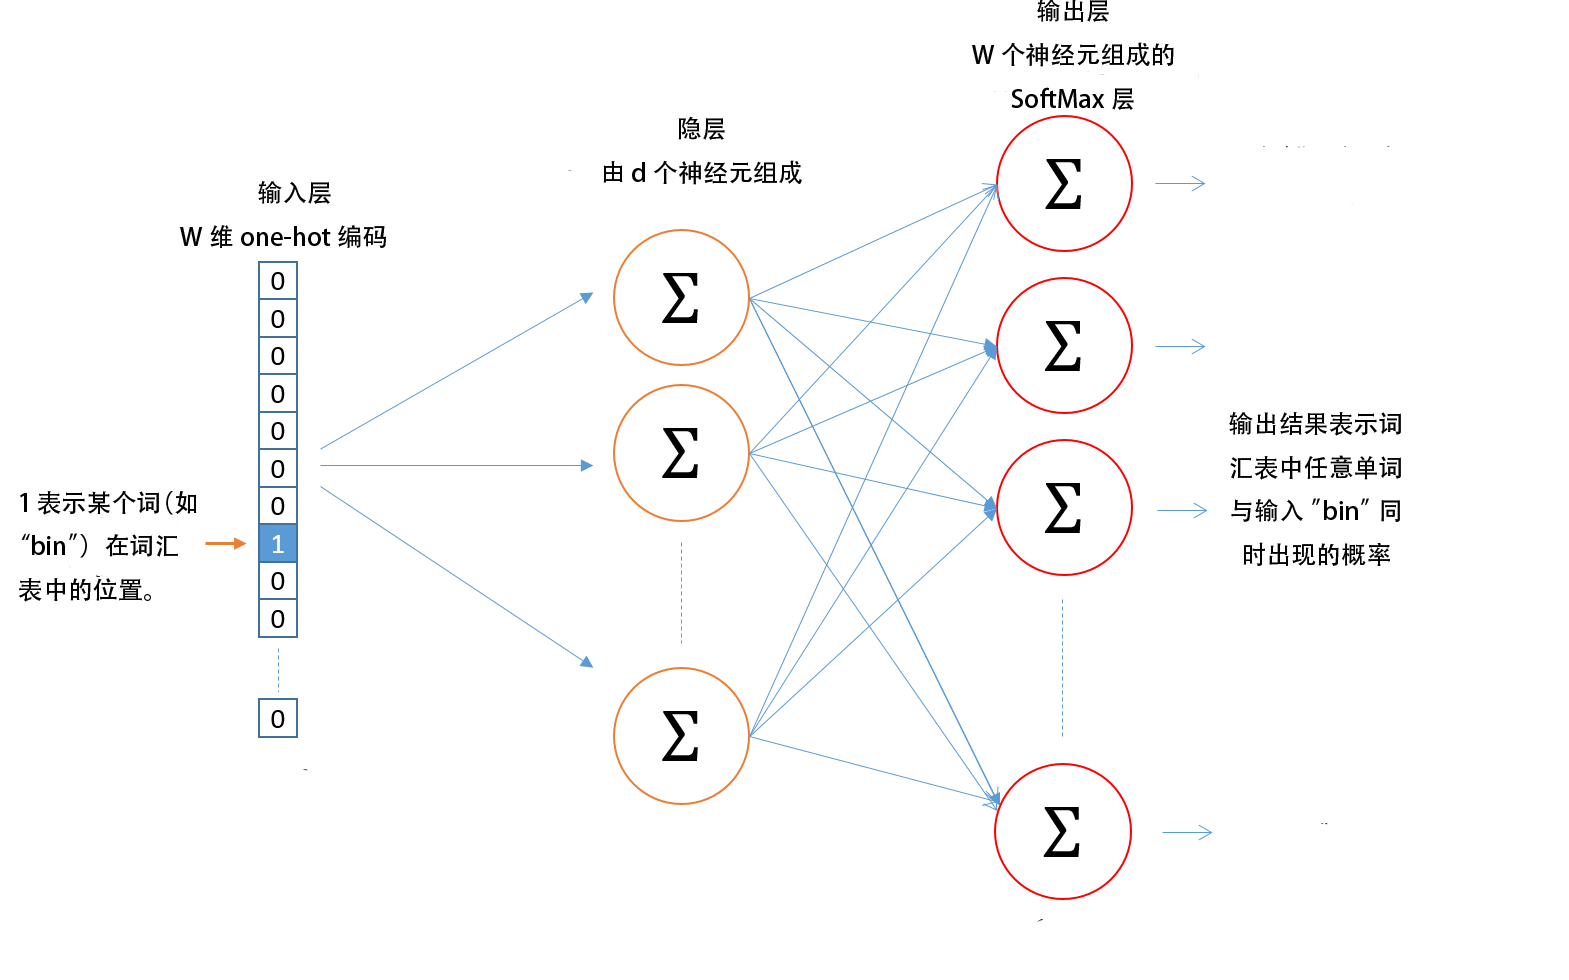
\includegraphics[width=\textwidth]{skip_gram_net_arch}
\caption{Skip-gram模型网络结构}
\label{fig:skip_gram_net_arch}
\end{figure}
如图\ref{fig:skip_gram_net_arch},
Skip-gram模型是一个三层神经网络,输入为词汇表中单词的初始向量,即$W$维的one-hot编码。隐层由$d$个神经元组成,没有激活函数,只有权值。训练收敛后隐层的$W\times d$的权值矩阵就是词汇表内所有词向量的集合。输出层为上文所述的softmax函数,最终结果是一个$W$维的向量,每个分量表示对应的单词与输入词存在上下文关系的概率。

当语料库规模较大,词汇表内单词较多时,采用softmax函数的计算复杂度过高。一种优化方式是使用层次化softmax(Hierarchical softmax)\cite{Hierarchical_softmax}。另一种计算复杂度更低,且同样能保证对原有softmax层拟合精度的优化方式是负采样(Negative sampling)。该方法将原来的预测上下文的问题转化为一系列独立的二分类问题,即,在选定中心词后,对词汇表中其他单词依次判定是否在中心词附近出现。


对任意中心词$\mathbf{w}_t$,用交叉熵损失函数(Cross-entropy Loss)代替原来的损失函数
\begin{equation}
    \label{eq:loss_of_t}
    L_t(\theta) = -\left( 
        \sum_{c \in \mathcal{C}_t} \log(p(\mathbf{w}_c | \mathbf{w}_t))+\sum_{c \in \mathcal{N}_t} \log(1-p(\mathbf{w}_c | \mathbf{w}_t)) 
    \right)
\end{equation}
其中$\mathcal{C}_t$表示中心词$w_t$的上下文单词集合(正样本),$\mathcal{N}_t$表示词汇表中,与$w_t$不存在上下文关系的单词(负样本)中随机抽取的若干噪声词。

由于任意单词与中心词是否上下文被视为独立事件,可用sigmoid函数拟合条件概率
\begin{equation}
    p(\mathbf{w}_c | \mathbf{w}_t) = \frac{1}{1+e^{-\mathbf{w}_t^{\top} \mathbf{w}_c}} = \sigma(\mathbf{w}_t^{\top} \mathbf{w}_c)
\end{equation}

代入\ref{eq:loss_of_t}并按$t$累加求平均,得到最终的损失函数:
\begin{equation}
    L(\theta) = -\frac{1}{T}\sum_{t=1}^{T} \left[
        \sum_{c \in \mathcal{C}_t} \log(\sigma(\mathbf{w}_t^{\top} \mathbf{w}_c)) + \sum_{c \in \mathcal{N}_t} \log(\sigma(-\mathbf{w}_t^{\top} \mathbf{w}_c))
    \right]
\end{equation}


%\begin{equation}
%    \label{eq:neg}
%    \log(1+e^{-\mathbf{w}_t^{\top} \mathbf{w}_c})+ \sum_{n \in \mathcal{N}_{t,c} }\log(1+ e^{\mathbf{w}_t^{\top} \mathbf{w}_n})
%\end{equation}
%
%
%用sigmoid函数$\sigma(x) = \log(1+e^{-x})$与公式\ref{eq:neg}代入目标函数\ref{eq:origin_object}得到最终的目标函数:
%\begin{equation}
%    \frac{1}{T} \sum_{t=1}^{T} \left[ \sum_{c \in \mathcal{C}_t} \sigma(\mathbf{w}_t^{\top} \mathbf{w}_c) + \sum_{n \in \mathcal{N}_{t,c}} \sigma(-\mathbf{w}_t^{\top} \mathbf{w}_n) \right]
%\end{equation}

经过以上优化后,Skip-gram模型训练的计算复杂度大大缩小。隐层的$W\times d$的权值矩阵$\theta$通过常规的随机梯度下降训练收敛后,作为最终词汇表$\mathcal{V}$的词向量模型。自此,该词汇表中的所有文件名或目录名\{ \textit{usr, bin, boot, ...}\}均可用$d$维向量表示。

3)完整路径的向量表示

\begin{figure}[htp]
\centering
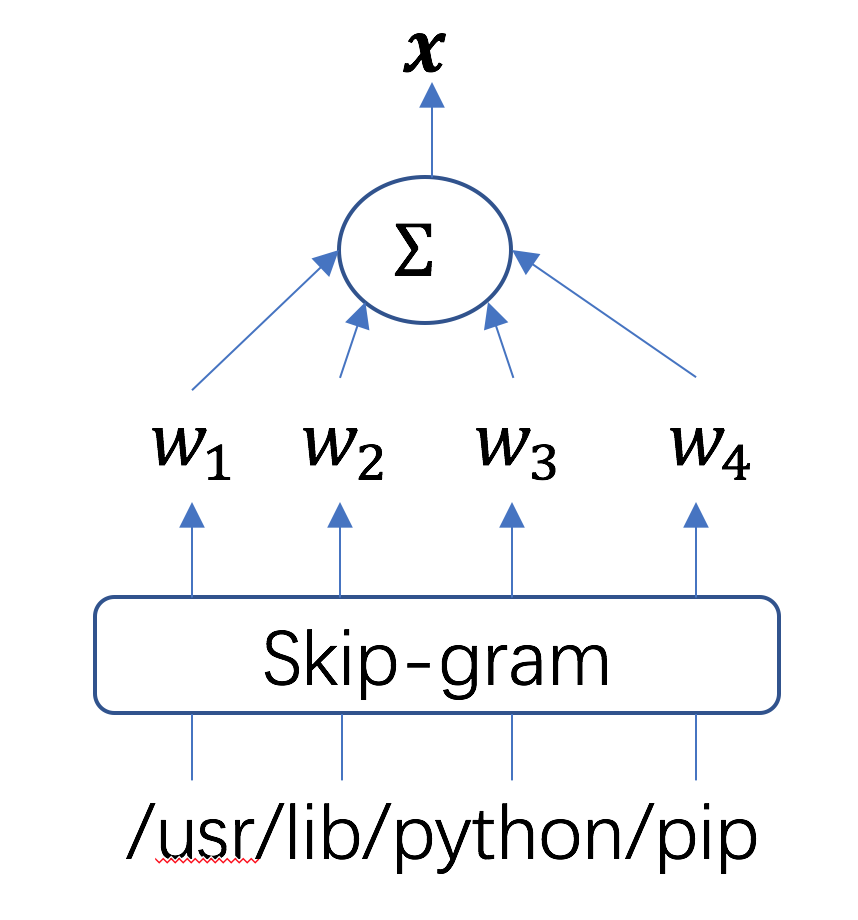
\includegraphics[width=.3\textwidth]{model_file_vec}
\caption{完整路径的向量表示}
\label{fig:model_file_vec}
\end{figure}
给定文件或目录(如/usr/lib/python/pip),每一级子目录对应的词向量$\mathbf{w_j}$被视为$d$维向量空间中的一段位移,将它们线性叠加得到该文件的向量表示($l$代表目录级数):

\begin{equation}
    \mathbf{x} = \sum_{j=1}^l \mathbf{w_j}
\end{equation}

\subsection{文件向量的降维可视化}

在文件与目录的词向量模型训练完成后,由于词向量的维度较高(本模型中维度$d$=100),本文使用主成分分析法(PCA,Principal Component Analysis)对生成的词向量进行降维与可视化,从而在直观上呈现不同文件名或目录名在语义上的相似性。

PCA是一种常见的数据分析方法,其主要目的是从词向量中找出最主要的特征,减少数据集维度的同时保持数据集中对方差影响最大的特征。换言之,PCA在原数据集中去除了重要性较低的特征,在原有信息损失较少的基础上将数据维度降低,以便于简化数据处理的计算复杂度或用于可视化。

在本模型中,词汇表$\mathcal{V}$生成的$W$条$d$维词向量组成矩阵$X$($d$行$W$列),采用PCA降成$k$维数据的处理步骤可简单概括如下:

1)将$X$的每一列进行零均值化处理,每个元素减去这一列的均值,使所有词向量各维度分量的均值为0。零均值化处理的作用是简化方差和协方差的计算。

2)求出协方差矩阵$C = \frac{1}{W} XX^{\top}$。$C$是一个对称矩阵,对角线元素$C_{ii}$表示所有词向量第$i$维分量的方差,$C_{ij}=C_{ji}$表示所有词向量第$i$维和第$j$维的协方差。

3)求出协方差矩阵的特征值与特征向量;

4)将特征向量按对应特征值大小从上到下按行排列成矩阵,取前$k$行组成矩阵$P$;

5)$Y=PX$就是降到$k$维后的数据。


\section{基于循环神经网络的热点数据识别}
\subsection{问题描述}
%设文件系统进行文件向量化处理后,所有文件向量($d$维)组成的集合记为$\mathcal{F} \subset \mathbb{R}^d$。在某工作负载的生命周期内对其文件访问进行追踪,将追踪日志转化为$d$维路径向量序列$\mathcal{S}=\{\mathbf{x}_1, \mathbf{x}_2,\dots, \mathbf{x}_T\}$。
%设上下文窗口大小为$N$,即
%在任意时刻$t$,追踪模块对前$N$次访问构成的日志序列$\{\mathbf{x}_{t-N+1}, \dots, \mathbf{x}_t\}$记为$\mathcal{L_t}$。
%定义该时刻的上下文序列$\mathcal{C}_t = \{ \mathbf{x}_{t-N+1}, \dots, \mathbf{x}_{t+N} \}$为正类样本(热文件),其余所有文件$\mathcal{N}_t = \mathcal{F} - \mathcal{C}_t$为负样本(冷文件)。
%
%在以上定义下,热点数据识别可转化为如下二分类问题的求解,其目标是:建立模型$M$,以$\mathcal{L}_t$为输入,计算这段访问序列所隐含的访问模式$\mathbf{h}_t$($d$维向量)。同时定义函数$f:\mathbb{R}^d \times \mathcal{F} \rightarrow [0,1]$,其含义为:访问模式$\mathbf{h}_t$下,文件$\mathbf{x}$是热点文件的概率。最后,为保证冷热文件的分类不会因为计算结果频繁扰动,设置合理的阈值$0<\alpha<\beta<1$来判定冷热。

设文件系统进行向量化表示后,所有文件向量组成的集合记为$\mathcal{F} \subset \mathbb{R}^d$。在某工作负载的生命周期内对其文件访问进行追踪,将追踪日志转化为文件向量序列$\mathcal{S}=\{\mathbf{x}_1, \mathbf{x}_2,\dots, \mathbf{x}_T\}$。

基于上述数据集,热点数据识别可转化为如下动态二分类问题求解:建立模型计算任意时刻$t$所隐含的访问模式$\mathbf{h}_t$。同时定义函数$f:\mathbb{R}^d \times \mathcal{F} \rightarrow [0,1]$,其含义为:访问模式$\mathbf{h}_t$下,文件$\mathbf{x}$是热点文件的概率。最后,为保证冷热文件的分类不会因为计算结果频繁扰动,设置合理的分类阈值$0<\alpha<1$来判定冷热。


\subsection{基于GRU神经网络的文件分类模型}
为了分析应用运行过程中产生的文件向量序列$\mathcal{S}=\{\mathbf{x}_1, \mathbf{x}_2,\dots, \mathbf{x}_T\}$,检测识别I/O行为特征,本文采用循环神经网络作为序列分析工具。
\begin{figure}[htp]
\centering
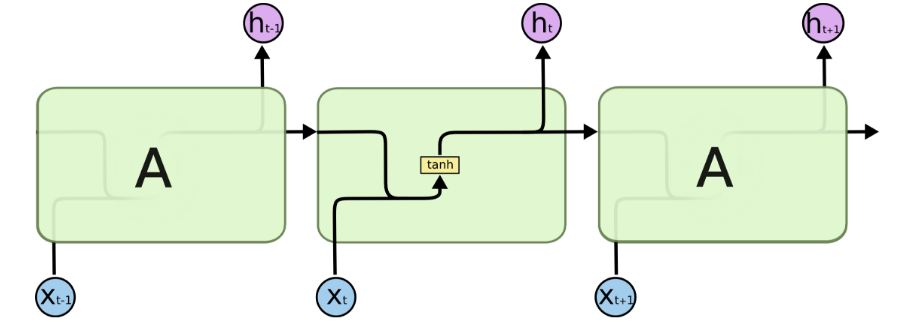
\includegraphics[width=\textwidth]{rnn_3}
\caption{使用单层全连接神经网络作为循环单元的RNN结构}
\label{fig:rnn_3}
\end{figure}

图\ref{fig:rnn_3}展示了一个最简单的循环神经网络,在这个循环体中只使用了一个类似全连接层的神经网络结构。下面将通过该图中所展示的神经网络来介绍循环神经网络前向传播的完整流程。

循环神经网络中的状态是通过一个向量来表示的,这个向量的维度也称为神经网络隐藏层的大小,设其为$h$。循环体中的神经网络的输入有两部分,一部分为上一时刻的状态$X_{t-1}$,另一部分为当前时刻的输入样本。对于时间序列数据来说,每一时刻的输入样例可以是当前时刻的数据;对于语言模型来说,输入样例可以是当前单词对应的词向量。
假设输入向量的维度为$x$,那么上图中循环体的全连接层神经网络的输入大小为$h+x$。也就是将上一时刻的状态与当前时刻的输入拼接成一个大的向量作为循环体中神经网络的输入。因为该神经网络的输出为当前时刻的状态,于是输出层的节点个数也为$h$(节点个数就是向量的维度,或者是隐藏层的大小),循环体中的参数个数为$(h+x)∗h+h(h+x)*h+h(h+x)∗h+h$个(这里可以理解为输入层有$h+x$个神经元,输出层有$h$个神经元,从而形成一个全连接的前馈神经网络,有$(h+x)*h$个权值,有$h$个偏置)。

同时循环体的神经网络输出不但提供给下一个时刻作为状态,同时还提供给当前的时刻作为输出。为了将当前时刻的状态转化为最终的输出,循环体还需要另外一个全连接神经网络来完成这个过程。这和卷积神经网络中最后的全连接层的意义是一样的。类似的,不同时刻用于输出的全连接神经网络中的参数也是共享的(参数一致)。

与常规神经网络相比,循环神经网络可以提取一段时间内文件访问序列的I/O行为特征,但上述简单神经元组成的循环神经网络面临着长期依赖(long-term dependencies)问题。在当前大数据背景下,海量小文件访问的读写性能是制约存储系统整体性能的瓶颈之一。此类应用在其生命周期内累积的访问序列长,依赖关系复杂,图\ref{fig:rnn_3}中给出的简单循环神经网络不具备处理长序列的能力。

长短期记忆网络(long short term memory, LSTM)\cite{LSTM}的设计正是为了解决上述RNN的长期依赖问题,是循环神经网络中里程碑式的网络结构设计。

\begin{figure}[htp]
\centering
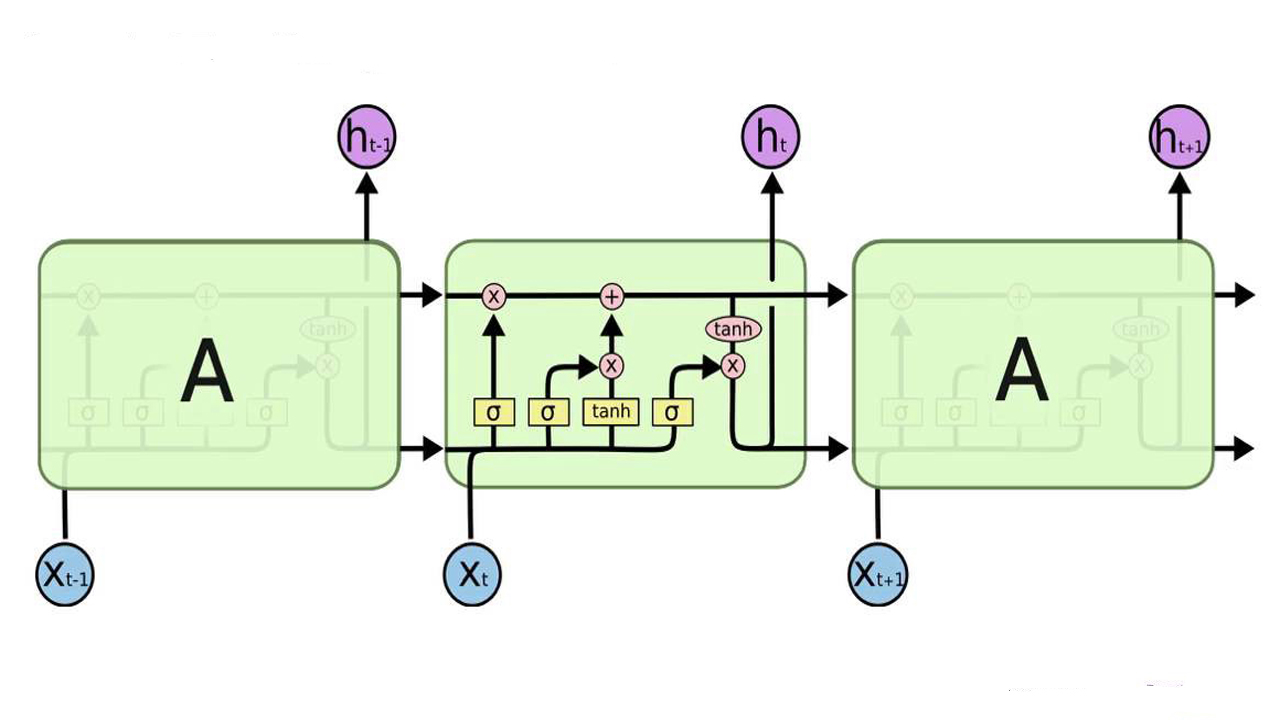
\includegraphics[width=\textwidth]{rnn_4}
\caption{长短期记忆网络LSTM}
\label{fig:rnn_4}
\end{figure}

LSTM的第一步是决定要从上一个时刻的状态中丢弃什么信息,其本质是由一个sigmoid全连接的前馈神经网络的输出管理,这种操作被称为遗忘门(forget get layer)。这个全连接的前馈神经网络的输入由向量$h_{t-1}$​和$x_t$组成,输出是$f_t$,1表示能够通过,0表示不能通过。
\begin{equation}
    f_t = \sigma(W_f \cdot [h_{t-1},x_t]+b_f)
\end{equation}

第二步决定哪些输入信息要保存到神经元的状态中。首先是一个sigmoid层的全连接前馈神经网络,称为输入门(input gate layer),其决定了哪些值将被更新;然后是一个tanh层的全连接前馈神经网络,其输出是一个向量$\tilde{C_t}$,该向量可以被添加到当前时刻的神经元状态中;最后根据两个神经网络的结果创建一个新的神经元状态。
\begin{align}
    i_t &= \sigma(W_i \cdot [h_{t-1,x_t}]+b_i) \\
    \tilde{C_t} &= \tanh(W_C \cdot [h_{t-1},x_t]+b_C)
\end{align}

第三步就可以上一时刻的状态$C_{t−1}$更新为当前状态$C_t$了。上述的第一步的遗忘门计算了一个控制向量,此时通过这个向量过滤一部分$C_{t-1}$状态;上述第二步的输入门根据输入向量计算了新状态,此时可以通过这个新状态$\tilde{C_{t-1}}$和$C_{t−1}$状态更新$C_t$
\begin{equation}
    C_t = f_t*C_{t-1} + i_t*\tilde{C_t}
\end{equation}
​	
最后一步就是决定神经元的隐状态$h_t$	,此时的输出根据上述第三步的状态$C_t$进行计算:首先通过sigmoid层生成一个过滤向量;然后通过一个$\tanh$函数计算当前时刻的$C_t$;最后通过sigmoid层输出当前时刻的输出。
\begin{align}
    o_t &= \sigma(W_o [h_{t-1},x_t]+b_o) \\
    h_t &= o_t * \tanh(C_t)
\end{align}

\begin{figure}[htp]
\centering
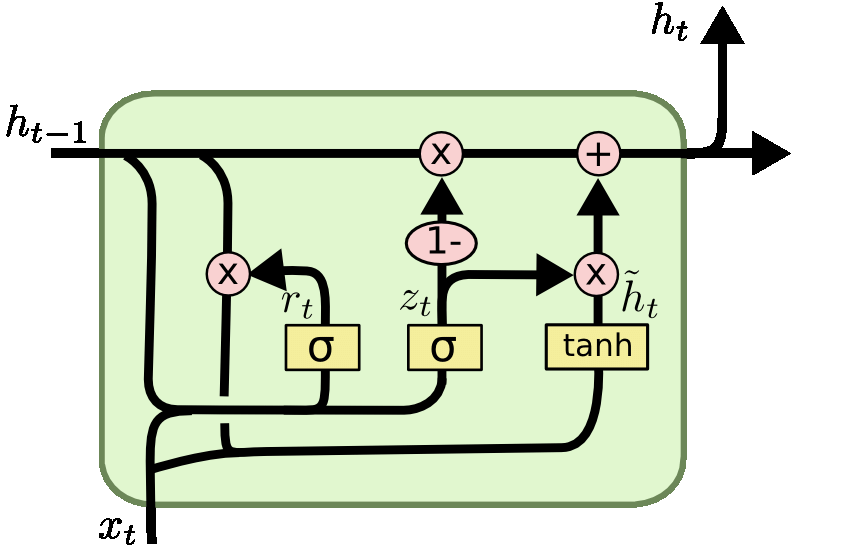
\includegraphics[width=0.6\textwidth]{gru}
\caption{GRU神经网络单元}
\label{fig:gru}
\end{figure}

GRU(Gated Recurrent Unit)\cite{GRU}是LSTM网络单元的一个变种。如图\ref{fig:gru}所示,GRU在解决长期依赖的基础上,将输入门、遗忘门和输出门缩减为更新门(update gate)和重置门(reset gate),结构更简单,训练与推断的计算复杂度更低。出于性能考虑,本文采用GRU作为I/O序列分析的网络单元。




1)输入层设计

设上下文窗口大小为$N$。在任意时刻$t$,我们将最近$N$次文件访问构成的日志序列$\{\mathbf{x}_{t-N+1}, \dots, \mathbf{x}_t\}$作为输入序列$\mathcal{L}_t$。

2)隐层设计

如图\ref{fig:gru},本文采用单层GRU来计算某一时刻隐含的文件访问模式$h_t$。前向传播的具体计算过程如下:

在时刻$t$, 我们用$h_t^{(j)}$来表示隐状态$\mathbf{h}_t$的第$j$个分量,由前一时刻隐状态$h_{t-1}^{(j)}$与候选隐状态$\tilde{h}_t^{(j)}$加权求和计算:
\begin{equation}
    h_t^{(j)} = (1-z_t^{(j)}) h_{t-1}^{(j)} + z_t^{(j)}\tilde{h}_t^{(j)},
\end{equation}
其中$z_t$为更新门(update gate),由当前时刻输入$\mathbf{x_t}$和上一刻的隐状态$\mathbf{h_{t-1}}$计算获得:
\begin{equation}
z_t^{(j)} = \sigma(W_z \mathbf{x}_t + U_z \mathbf{h}_{t-1})^{(j)}
\end{equation}
候选隐状态$\tilde{h}_t^{(j)}$的计算如下:
\begin{equation}
    \tilde{h}_t^{(j)} = \tanh(W \mathbf{x}_t + U (\mathbf{r}_t \odot \mathbf{h}_{t-1}))^{(j)}
\end{equation}
此处$\mathbf{r}_t$是重置门(reset gate),运算符号$\odot$表示行列相同的矩阵之间的逐元素相乘(Hadamard product)。此处表示$\mathbf{r}_t$的第$j$个元素与隐状态$h_{t-1}$的第$j$个元素相乘。

重置门$r_t$由以下表达式求得:
\begin{equation}
    r_t^{(j)} = \sigma(W_r \mathbf{x}_t + \mathbf{U}_r \mathbf{h}_{t-1})^{(j)}
\end{equation}

3)输出层设计

如上文所述,我们构造了单层GRU来计算隐状态$h_t$,为了赋予$h_t$识别热点文件的功能,我们构造函数$f:\mathbb{R}^d \times \mathcal{F} \rightarrow [0,1]$用于计算在状态$\mathbf{h}_t$下,文件$\mathbf{x}_t$是热数据的条件概率:
\begin{align}
    \begin{split}
    p(\mathbf{x} | \mathbf{h}_t) &= f(\mathbf{h}_t,\mathbf{x}) \\
                                &= \sigma(\mathbf{h}_t^{\top} \mathbf{x}) \\
                                &= \frac{1}{1+e^{-\mathbf{h}_t^{\top} \mathbf{x}}}
    \end{split}
\end{align}

与常规的文本分类任务不同,文件访问序列组成的样本不带标签,或者说冷、热标签是随着时刻$t$动态改变的。在实际应用场景下,$t$时刻前访问尚未结束的文件,以及接下来即将访问的文件都是热数据,然而缓存容量是有限的,可以被纳入热数据的总量应与缓存容量呈正相关。为简化模型起见,此处设定与时间无关,只与缓存容量相关的超参数$M$,将文件序列$\{ x_{t-M+1},\dots,x_t,\dots,x_{t+M} \}$共计$2*M$条文件标记为正类样本集$C_t$,其余文件为冷数据。

通常冷文件数量近似于文件总数$|\mathcal{F}|$,考虑到实际文件系统中总文件数量巨大,将所有冷文件纳入负类样本将带来巨大的计算量。为此,本文借鉴Skip-gram算法中采用的负采样(Negtive sampling)的思想,对冷文件集随机采集$K$个样本组成负类样本集$\mathcal{N}_t$。

为训练该模型,采用二分类最常用的交叉熵损失函数:
\begin{equation}
    L(\theta) = \frac{1}{T-2M}\sum_{t=M}^{T-M+1} \left[
        \sum_{\mathbf{x} \in \mathcal{C}_t} \log(\sigma(\mathbf{h}_t^{\top} \mathbf{x}) + 
        \sum_{\mathbf{x} \in \mathcal{N}_t} \log(-\sigma(\mathbf{h}_t^{\top} \mathbf{x})
    \right]
\end{equation}

其中,待训练的参数$\theta$为GRU中各个部件的权重矩阵$W_z, U_z, W, U, W_r, U_r$,训练采用时序后向传播算法(Backpropagation Through Time)。要设置和调优的超参数包括输入序列长度$N$,与缓存容量正相关的热文件样本数$M$,以及负样本采样数$K$。

结合上节介绍的基于Skip-gram的文件向量模型,整体设计框架如图\ref{fig:skip_gram_gru}。

\begin{figure}[htp]
\centering
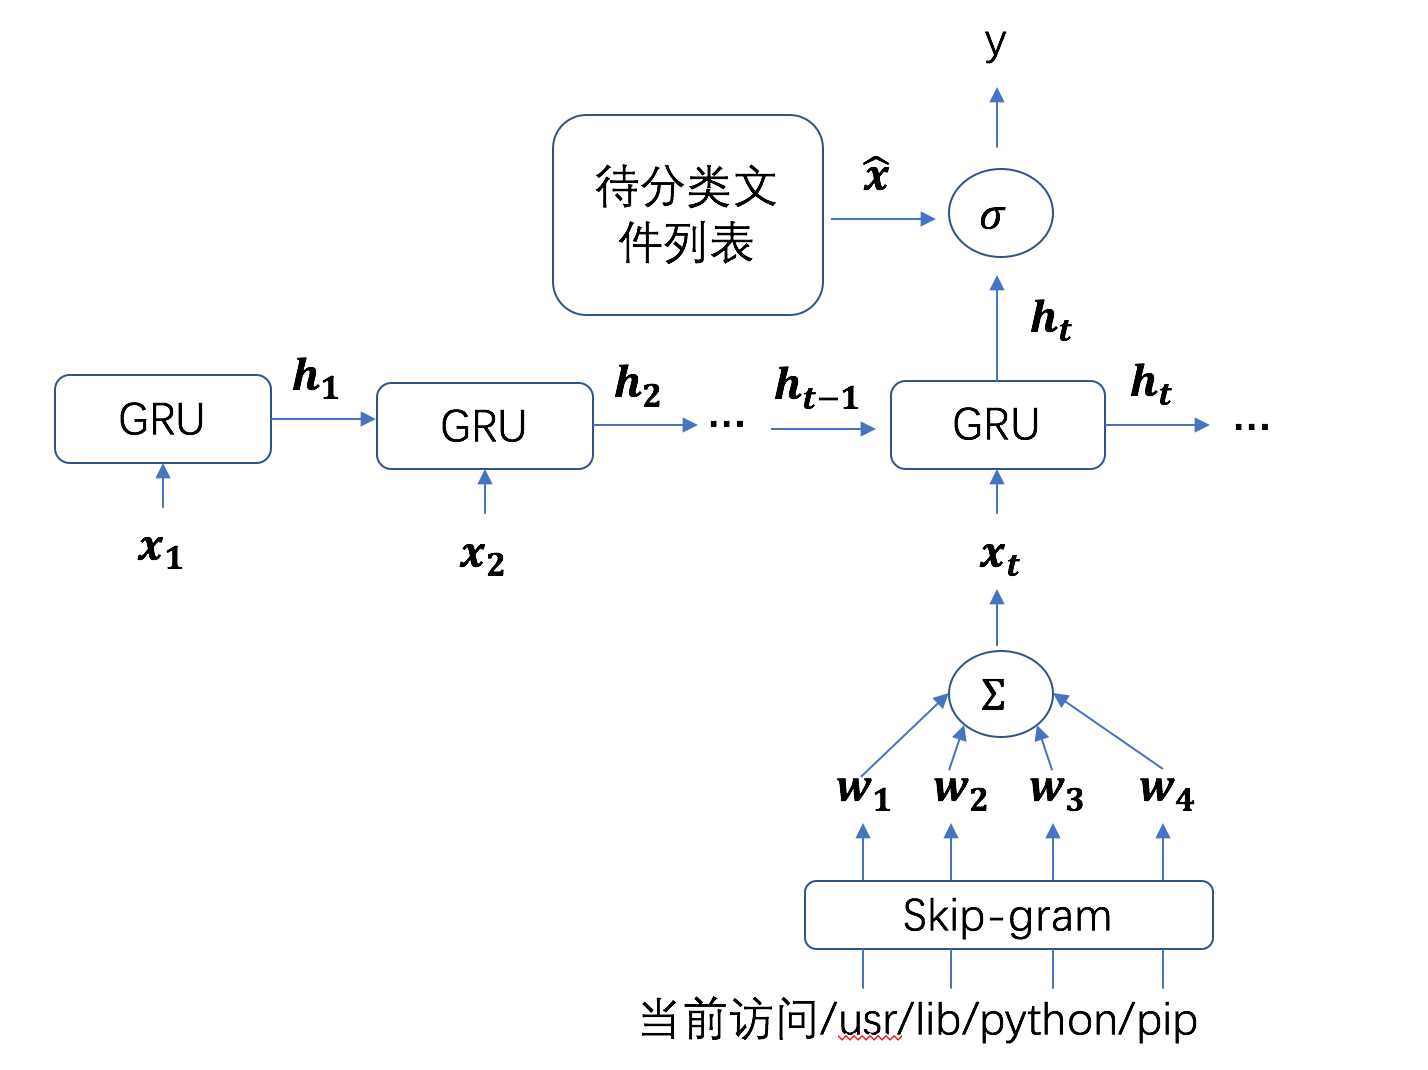
\includegraphics[width=.8\textwidth]{skip_gram_gru}
\caption{文件分类模型网络结构}
\label{fig:skip_gram_gru}
\end{figure}


%指标以命中率、错判率为主,即准确率召回率?
\section{本章小结}
目前分层存储管理优化方式主要包括两方面:一是挖掘文件的关联性(Block Correlation),二是动态追踪应用的I/O行为并加以分析,实现I/O行为预测(热数据识别),以指导数据迁移模块进行主动的数据预取和缓存替换。以往的研究具有局限性,例如,对文件的关联性挖掘局限于目录树结构表现出的文件关系,没有对文件或目录命名隐含的语义关系予以分析;I/O 行为的分析通常只针对短期内的访问规律,没有在长时间跨度上进行分析。为解决上述问题,探索新的分层管理优化方式,本章设计了以下两个模型:

1)基于词嵌入模型的文件向量化表示。数据块关联(Block Correlation)在文件系统中广泛存在,且这种数据间的联 系通常比较稳定,在目录结构不发生变化的情况下,一般不受工作负载的运行状 态影响。反过来,工作负载访问文件的部分规律是由文件之间的固有关系决定的。 如果能显示地挖掘出文件之间的联系,可以为存储系统的数据分布策略、迁移策 略等提供帮助。本文从文件之间语义关系入手,建立了词嵌入模型将文件和目录映射为向量,将文件之间的关联分析转化为向量运算。

2)基于循环神经网络的文件分类模型。本文对冷热文件分类任务进行了形式化定义,在文件向量化表示的基础上,建立了GRU循环神经网络对应用的I/O序列进行分析和文件分类。



